\documentclass[10pt]{beamer}

%%%
% PREAMBLE FOR THIS DOC 
%%%
%https://tex.stackexchange.com/questions/68821/is-it-possible-to-create-a-latex-preamble-header
\usepackage{/Users/miw267/Repos/csci246_spring2025/slides/preambles/beamer_preamble_for_CSCI246}



%%% TRY TO RESHOW TOC AT EACH SECTION START (with current section highlighted)
% Reference: https://tex.stackexchange.com/questions/280436/how-to-highlight-a-specific-section-in-beamer-toc
\newcommand\tocforsect[2]{%
  \begingroup
  \edef\safesection{\thesection}
  \setcounter{section}{#1}
  \tableofcontents[#2,currentsection]
  \setcounter{section}{\safesection}
  \endgroup
}


%%%% HERES HOW TO DO IT CORRECTLY
% FIRST IN .STY FILE, DO
%\usetheme[sectionpage=none]{metropolis}
% THEN AT EACH SECTION DO
%\begin{frame}{Outline}
%  \tableofcontents[currentsection]	
%\end{frame}



%\setbeamertemplate{navigation symbols}{}
%\setbeamertemplate{footline}[frame number]{}


%%%
% DOCUMENT
%%%

\begin{document}

%\maketitle

%% Title page frame
%\begin{frame}
%    \titlepage 
%\end{frame}





\title{Wednesday 01/22/2025: Proofs}
\author{CSCI 246: Discrete Structures}
\date{Textbook reference: Sec. 5, Scheinerman}

\begin{frame}
    \titlepage 
\end{frame}


\begin{frame}{Announcements before today's quiz}

\begin{itemize}
\item \textbf{Sheet of paper}: Please bring your own sheet of paper to class each day for quizzes if possible. However, if you don't have any, you are welcome to take a blank sheet of paper from the stack in the front of the room.
\item \textbf{Rules for quizzes}: For all quizzes in the course, you should use only paper and pencil.  Please close your computers and textbooks, and put away your cellphones.    
\end{itemize}


\end{frame}


\begin{frame}{Reading Quiz}

\vfill 

 \begin{quiz}[title=Quiz Question]
Prove that the the sum of two even integers is even.\\
Use the appropriate proof template from the textbook. 
\end{quiz}

\pause 


\vfill \vfill 

%You may want to use the following definitions.


\begin{mydef}[title=Definition 3.1 (\textbf{Even})]
An integer is called \textit{even} provided it is divisible by two.
\end{mydef}

\begin{mydef}[title=Definition 3.2 (\textbf{Divisible})]
Let $a$ and $b$ be integers.  We say that $a$ is \textit{divisible} by $b$ provided there is an integer $c$ such that $bc=a$.  We also say that $b$ \textit{divides} $a$, or $b$ is a \textit{factor} of $a$, or $b$ is a \textit{divisor} of $a$.  The notation for this is $b|a$. 
\end{mydef}

\end{frame}



\begin{frame}{Solution Sketch}
\textbf{Proposition.} The sum of two even integers is even.

\textbf{Proof.}

\begin{tabularx}{\textwidth}{|L{3cm}|X|}
\hline \textbf{Annotation} & \textbf{Main Text} \\ \hline
 \hlorange{Convert Prop. to ``if-then" form} &  \hlorange{We show that if $x$ and $y$ are even integers, then $x+y$ is even.} \\ \hline
\hlblue{State ``if"} & \hlblue{Let $x$ and $y$ be even integers} \\ \hline
\hlgreen{Unravel defs.} & \hlgreen{Then by Defs. 3.1 and 3.2, there exist integers $a,b$ such that $x=2a$ and $y=2b$.} \\ \hline
\hlred{*** The glue ***} & \hlred{What goes here?!?!} \\ \hline
 \hlgreen{Unravel defs.} & \hlgreen{So there is an integer $c$ such that $x+y=2c$.} \\ \hline
  \hlblue{State ``then"} & \hlblue{Hence, $x+y$ is even.} \\ \hline
\hline
\end{tabularx}
\end{frame}


\begin{frame}{Solution}
\textbf{Proposition.} The sum of two even integers is even.

\textbf{Proof.}

\begin{tabularx}{\textwidth}{|L{3cm}|X|}
\hline \textbf{Annotation} & \textbf{Main Text} \\ \hline
 \hlorange{Convert Prop. to ``if-then" form} &  \hlorange{We show that if $x$ and $y$ are even integers, then $x+y$ is even.} \\ \hline
\hlblue{State ``if"} & \hlblue{Let $x$ and $y$ be even integers} \\ \hline
\hlgreen{Unravel defs.} & \hlgreen{Then by Defs. 3.1 and 3.2, there exist integers $a,b$ such that $x=2a$ and $y=2b$.} \\ \hline
\hlred{*** The glue ***} &   \hlred{Hence, $x+y = 2a+2b = 2(a+b)$.} \\ \hline
 \hlgreen{Unravel defs.} & \hlgreen{So there is an integer $c=a+b$ such that $x+y=2c$.} \\ \hline
  \hlblue{State ``then"} & \hlblue{Hence, $x+y$ is even.} \\ \hline
\hline
\end{tabularx}
\end{frame}



\begin{frame}{General announcements}
\begin{itemize}
\item \textbf{Course repo}: Can navigate to syllabus (updated with TA/tutoring hours) and slides (e.g. group exercises with solutions).  Both are mutable. Url is in Brightspace if you forget.    
\item \textbf{Brightspace email question}: Sometimes will send a message (e.g. survey response) in Brightspace email. Is that something you see?
\item \textbf{Roster Logistics}: Drew Bolster please come see me after class. 
\item \textbf{Friday's problems quiz}:  Although the group exercises are done collaboratively in groups of 3 people, the "problems quizzes": on Fridays will be taken by individuals.  It will be combined with the reading quiz and can be done the same sheet of paper.
\end{itemize}
% Who is Drew Bolster (not on roster but received a quiz). Ask to come up after class.
	
\end{frame}

\begin{frame}{Sec 4. Reading Quiz Scores}

\begin{figure}
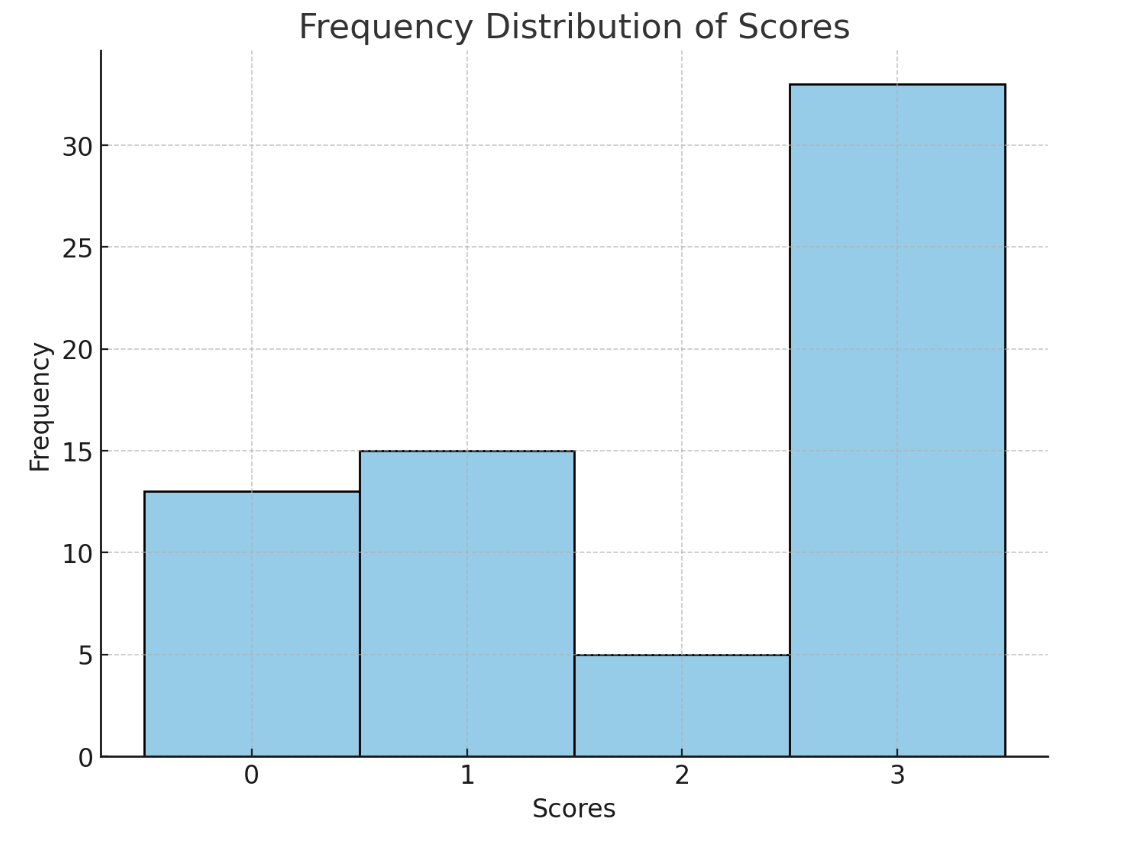
\includegraphics[width=0.7\textwidth]{images/sec4_scores.png}
\end{figure}

\footnotesize 
%
What to conclude if your score was lower than you wanted?
\begin{itemize}
\item \textbf{Growth mindset}: \greencheck  Abilities are malleable and capable of improvement with effort.  (e.g. "I need to change my reading strategy.") 
\item \textbf{Fixed mindset}: \redx  Abilities are fixed and unchangeable. (e.g. "I'm not smart/a math person/a good test taker.")	
\end{itemize}
%
\end{frame}

\begin{frame}[standout]

\vfill 
\alert{Review solutions to Sec. 4 group exercises}
\vfill

\end{frame}



\begin{frame}[standout]

\alert{Sec. 5 group work!}
\vfill
Students are randomly assigned into groups of 3 on the next slide.
\vfill 
Each group gets $\half$ of a white board.
\vfill
If the  $\half$ white board is inconvenient, feel free to write on a window! 
\end{frame}

\begin{frame}
\footnotesize
Group 1: bridger.voss,connor.mizner,nolan.scott1\\
Group 2: john.fotheringham,william.elder1,justice.mosso\\
Group 3: ethan.johnson18,michael.oswald,lynsey.read\\
Group 4: aaron.loomis,conner.reed1,luke.donaldson1\\
Group 5: griffin.short,joseph.triem,caitlin.hermanson\\
Group 6: joseph.mergenthaler,reid.pickert,yebin.wallace\\
Group 7: erik.moore3,samuel.rollins,james.brubaker\\
Group 8: jacob.shepherd1,connor.graville,connor.yetter\\
Group 9: zeke.baumann,ryan.barrett2,jada.zorn\\
Group 10: peyton.trigg,jakob.kominsky,jonas.zeiler\\
Group 11: jett.girard,jacob.ketola,carver.wambold\\
Group 12: emmeri.grooms,nicholas.harrington1,lucas.jones6\\
Group 13: blake.leone,tyler.broesel,sarah.periolat\\
Group 14: luka.derry,anthony.mann,pendleton.johnston\\
Group 15: peter.buckley1,jack.fry,cameron.wittrock\\
Group 16: samuel.hemmen,jacob.ruiz1,derek.price4\\
Group 17: jeremiah.mackey,matthew.nagel,devon.maurer\\
Group 18: micaylyn.parker,samuel.mosier,owen.obrien\\
Group 19: mason.barnocky,alexander.goetz,carsten.brooks\\
Group 20: adam.wyszynski,timothy.true,joseph.windmann\\
Group 21: evan.barth,alexander.knutson,tristan.nogacki\\
Group 22: julia.larsen,evan.schoening,colter.huber\\
Group 23: delaney.rubb,kaden.price
\end{frame}


\begin{frame}{Group exercises}
\begin{enumerate}
	\item Prove that the square of an odd integer is odd.
	\item Prove that the difference between consecutive perfect squares is odd.
	\item Let $x$ be an integer.  Prove that $0|x$ if and only if $x=0$.
	\item Prove that an integer is odd if and only if it is the sum of two consecutive integers.
\end{enumerate}
	
\end{frame}


\begin{frame}{Group exercise \#1: Solution}
\textbf{Proposition.} The square of an odd integer is odd.

\textbf{Proof.}

\begin{tabularx}{\textwidth}{|L{3cm}|X|}
\hline \textbf{Annotation} & \textbf{Main Text} \\ \hline
 \hlorange{Convert Prop. to ``if-then" form} &  \hlorange{We show that if $x$ is an odd integer, then $x^2$ is odd.} \\ \hline
\hlblue{State ``if"} & \hlblue{Let $x$ be an odd integer.} \\ \hline
\hlgreen{Unravel defs.} & \hlgreen{Then by definition of \textit{odd}, there is an integer $a$ such that $x=2a+1$.} \\ \hline
\hlred{*** The glue ***} &   \hlred{So $x^2= (2a+1)(2a+1) = 4a^2+4a+1 = 2 (2a^2+2a) +1$.} \\ \hline
 \hlgreen{Unravel defs.} & \hlgreen{So there is an integer $b$ \red{(where $b=2a^2+2a$)} such that $x^2=2b+1$.} \\ \hline
  \hlblue{State ``then"} & \hlblue{Hence, $x^2$ is odd.} \\ \hline
\hline
\end{tabularx}
\pause 
\vfill 
\footnotesize 
\textbf{Remark.}  You do not need to provide the annotations or colors in your own proofs. I am using them here in the solution to highlight the formulaic structure of an if-then proof.
\end{frame}

\begin{frame}{Group exercise \#2: Solution}
\textbf{Proposition.} The difference between consecutive perfect squares is odd.

\textbf{Proof.}

\begin{tabularx}{\textwidth}{|L{3cm}|X|}
\hline \textbf{Annotation} & \textbf{Main Text} \\ \hline
 \hlorange{Convert Prop. to ``if-then" form} &  \hlorange{We show that if $x$ and $y$ are consecutive perfect squares, then $x-y$ is odd. } \\ \hline
\hlblue{State ``if"} & \hlblue{Let $x$ and $y$ be consecutive perfect squares} \\ \hline
\hlgreen{Unravel defs.} & \hlgreen{Then $x=(z+1)^2$ and $y=z^2$ where $z$ is an integer.} \\ \hline
\hlred{*** The glue ***} &   \hlred{So $x-y= (z+1)^2 - z^2 = (z^2 + 2z +1) -z^2  = 2z+ 1$.} \\ \hline
 \hlgreen{Unravel defs.} & \hlgreen{So there is an integer $b$ \red{(where $b=z$)} such that $x-y=2b+1$.} \\ \hline
  \hlblue{State ``then"} & \hlblue{Hence, $x-y$ is odd.} \\ \hline
\hline
\end{tabularx}
\pause 
\vfill 
\footnotesize 
\textbf{Remark.}  You do not need to provide the annotations or colors in your own proofs. I am using them here in the solution to highlight the formulaic structure of an if-then proof.
\end{frame}

\begin{frame}{Group exercise \#3: Solution}
\small 
\textbf{Proposition.} Let $x$ be an integer.  Prove that $0|x$ if and only if $x=0$.

\textbf{Proof.} We decompose the \textit{if-and-only-if} statement into two \textit{if-then} statements.

\begin{itemize}
\item[(a)] \hlorange{We show that if $0|x$, then $x=0$.} \hlblue{Let $x$ be an integer such that $0|x$.}  \hlgreen{Then by definition of \textit{divisible}, there is an integer $a$ such that $0 \cdot a = x$.}  \hlred{But $0 \cdot a = 0$.}  \hlblue{Hence $x=0$.}
\item [(b)]  \hlorange{We show that if $x=0$, then $0|x$.} \hlblue{Let $x=0$.} \hlred{Let $a$ be any integer. (For example, take $a=7$.)  Then $a \cdot 0 =0$.}  \hlgreen{Hence, there is an integer $a$ such that $0 \cdot a = x$.} \hlblue{Hence, $0|x$.}  	
\end{itemize}
\pause 
\vfill 
\textbf{Remark.} An \textit{if-and-only-if} proof consists of two \textit{if-then} proofs. Each uses the same \textit{if-then} template (and same color-scheme) as in Group Exercises \#1 and \#2.   Note that some green rows were skipped (as there was no definition to unravel for $x=0$).
\end{frame}

\begin{frame}{Group exercise \#4: Solution}
\footnotesize 
\textbf{Proposition.}
An integer is odd if and only if it is the sum of two consecutive integers.
 
\textbf{Proof.} We decompose the \textit{if-and-only-if} statement into two \textit{if-then} statements.

\begin{itemize}
\item [(a)]  \hlorange{We show that if $x$ is the sum of two consecutive integers, then $x$ is an odd integer.} \hlblue{Let $x$ be the sum of two consecutive odd integers.}  \hlgreen{So there is an integer $a$ such that $x= a + (a+1)$.} \hlred{So $x=2a+1$}  \hlgreen{Hence, there is an integer $a$ such that $x = 2a+1$.} \hlblue{Hence, $x$ is an odd integer.}  	
\item[(b)] \hlorange{We show that if $x$ is an odd integer, then $x$ is the sum of two consecutive integers.} \hlblue{Let $x$ be an odd integer.}  \hlgreen{Then by definition of \textit{odd}, there is an integer $a$ such that $x=2a+1$.}  \hlred{So we have $x=2a+1 = a + (a+1)$.}  \hlblue{Hence $x$ is the sum of two consecutive integers.}
\end{itemize}

\pause 
\vfill 
\textbf{Remark.} An \textit{if-and-only-if} proof consists of two \textit{if-then} proofs. Each uses the same \textit{if-then} template (and same color-scheme) as in Group Exercises \#1 and \#2. 
\end{frame}



\end{document}
